
\section{Convergence Test Examples}


\subsection{Dahlquist Test Equation\label{rythmos:sec:Dahlquist-Test}}

The Dahlquist Test equation,
\begin{equation}
\dot{x}=\lambda x,\label{rymthos:eq:Dahlquist-Test}
\end{equation}
is used to investigate and classify the properties of integrators.
Its solution is $x=ce^{\lambda t}$ where $\lambda$ can be complex
with positive, negative coefficients, and provides a variety of canonical
problems (\emph{e.g.}, exponentially increasing and decaying solutions,
and oscillatory solutions). By implementing time integrators in the
Dahlquist test equation, the amplification or stability factor, $R(z)$,
can be determined by writing it in the update form
\[
x_{n}=R(\lambda\Delta t)\, x_{n-1}=R(z)\, x_{n-1}
\]
where $z=\lambda\Delta t$. A few important measures of stability
are absolute stability, A-stability and L-stability and are defined
by $z$ and $R(z)$. First off, absolute stability requires the solution
has no growth from one time step to the next, 
\[
\left|x_{n}\right|\leq\left|x_{n-1}\right|
\]
and this true when
\[
\left|R(z)\right|\leq1
\]
which defines the stability domain. A-stable methods have a stability
domain for the negative half domain where $Re(z)\leq0$. Although
A-stability is useful for many non-stiff equations, stiff equations
require additional stability properties to A-stability, $\left|R(z)\right|\rightarrow0$
as $z\rightarrow-\infty$, and is known as L-stability.


\subsection{SinCos Problem\label{rythmos:sec:SinCos-Problem}}

This is a canonical Sine-Cosine differential equation
\[
\mathbf{\ddot{x}}=-\mathbf{x}
\]
with a few enhancements. We start with the exact solution to the differential
equation 
\begin{eqnarray*}
x_{0}(t) & = & a+b*\sin((f/L)*t+\phi)\\
x_{1}(t) & = & b*(f/L)*\cos((f/L)*t+\phi)
\end{eqnarray*}
then the form of the model is: 
\begin{eqnarray*}
\frac{d}{dt}x_{0}(t) & = & x_{1}(t)\\
\frac{d}{dt}x_{1}(t) & = & \left(\frac{f}{L}\right)^{2}(a-x_{0}(t))
\end{eqnarray*}
where the default parameter values are $a=0$, $f=1$, and $L=1$,
and the initial conditions
\begin{eqnarray*}
x_{0}(t_{0}=0) & = & \gamma_{0}[=0]\\
x_{1}(t_{0}=0) & = & \gamma_{1}[=1]
\end{eqnarray*}
determine the remaining coefficients
\begin{eqnarray*}
\phi & = & \arctan(((f/L)/\gamma_{1})*(\gamma_{0}-a))-(f/L)*t_{0}[=0]\\
b & = & \gamma_{1}/((f/L)*cos((f/L)*t_{0}+\phi))[=1]
\end{eqnarray*}
The solution is shown in Fig.~\ref{rythmos:fig:SinCos-exact}. 
\begin{figure}


\begin{centering}
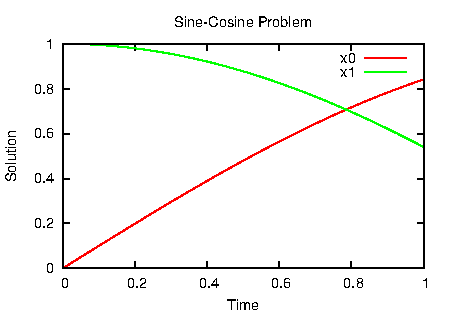
\includegraphics{figures/sincos}\caption{Exact solution to the Sine-Cosine problem.\label{rythmos:fig:SinCos-exact}}

\par\end{centering}

\end{figure}
Therefore this model has three model parameters and two initial conditions
which effect the exact solution as above. 
\[
\mathbf{p}=(a,f,L)
\]
\[
\dot{\mathbf{x}}=\mathbf{F}(\mathbf{x},t,\mathbf{p})
\]
where
\begin{eqnarray*}
F_{0} & = & x_{1}\\
F_{1} & = & \left(\frac{f}{L}\right)^{2}(a-x_{0})
\end{eqnarray*}


The exact sensitivities, $\mathbf{s}=\partial\mathbf{x}/\partial\mathbf{p}$,
for the problem are specified as
\[
\mathbf{s}(t)=\left[\begin{array}{cc}
1 & 0\\
\left(\frac{b}{L}\right)t\,\cos\left(\left(\frac{f}{L}\right)t+\phi\right) & \left(\frac{b}{L}\right)\cos\left(\left(\frac{f}{L}\right)t+\phi\right)-\frac{b\, f\, t}{L^{2}}\sin\left(\left(\frac{f}{L}\right)t+\phi\right)\\
-\frac{b\, f\, t}{L^{2}}\cos\left(\left(\frac{f}{L}\right)t+\phi\right) & -\frac{b\, f}{L^{2}}\cos\left(\left(\frac{f}{L}\right)t+\phi\right)+\frac{b\, f^{2}\, t}{L^{3}}\sin\left(\left(\frac{f}{L}\right)t+\phi\right)
\end{array}\right]
\]
and for the default initial conditions, $\phi=0$ and $b=1$
\[
\mathbf{s}(t=0)=\left[\begin{array}{cc}
1 & 0\\
0 & \frac{b}{L}\\
0 & -\frac{f}{L^{2}}
\end{array}\right]
\]
The time differentiated sensitivities, $\dot{\mathbf{s}}=\partial\mathbf{s}/\partial t=\partial/\partial t(\partial\mathbf{x}/\partial\mathbf{p})=\partial/\partial\mathbf{p}(\partial\mathbf{x}/\partial t)$
are
\[
\dot{\mathbf{s}}(t)=\left[\begin{array}{cc}
0 & 0\\
\left(\frac{b}{L}\right)\cos\left(\left(\frac{f}{L}\right)t+\phi\right)-\frac{b\, f\, t}{L^{2}}\sin\left(\left(\frac{f}{L}\right)t+\phi\right) & -\frac{2b\, f}{L^{2}}\sin\left(\left(\frac{f}{L}\right)t+\phi\right)\left(\frac{b}{L}\right)-\frac{b\, f^{2}\, t}{L^{3}}\cos\left(\left(\frac{f}{L}\right)t+\phi\right)\\
-\frac{b\, f}{L^{2}}\cos\left(\left(\frac{f}{L}\right)t+\phi\right)+\frac{b\, f^{2}\, t}{L^{3}}\sin\left(\left(\frac{f}{L}\right)t+\phi\right) & \frac{2b\, f^{2}}{L^{3}}\sin\left(\left(\frac{f}{L}\right)t+\phi\right)+\frac{b\, f^{3}\, t}{L^{4}}\cos\left(\left(\frac{f}{L}\right)t+\phi\right)
\end{array}\right]
\]



\subsection{Log-Time Problem\label{rythmos:sec:Log-Time-Problem}}

This problem was generated to be similar to those seen in Charon.
What is different about this solution is that it evolves on logarithmic
scale. As seen in Fig.~\ref{rythmos:fig:LogTime-exact}, the solution
has a very sharp gradient near $t=10^{-9}$ and then decays over many
order of magnitude until near constant at $t=1$.
\begin{figure}
\centering{}%
\begin{tabular}{cc}
a)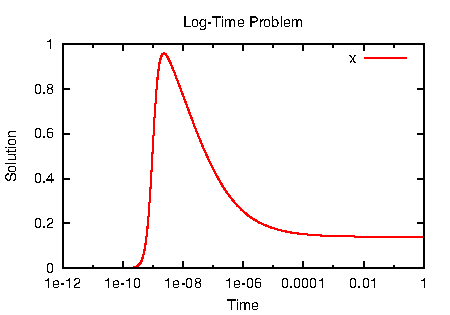
\includegraphics[width=2.75in]{figures/logtime-log} & b)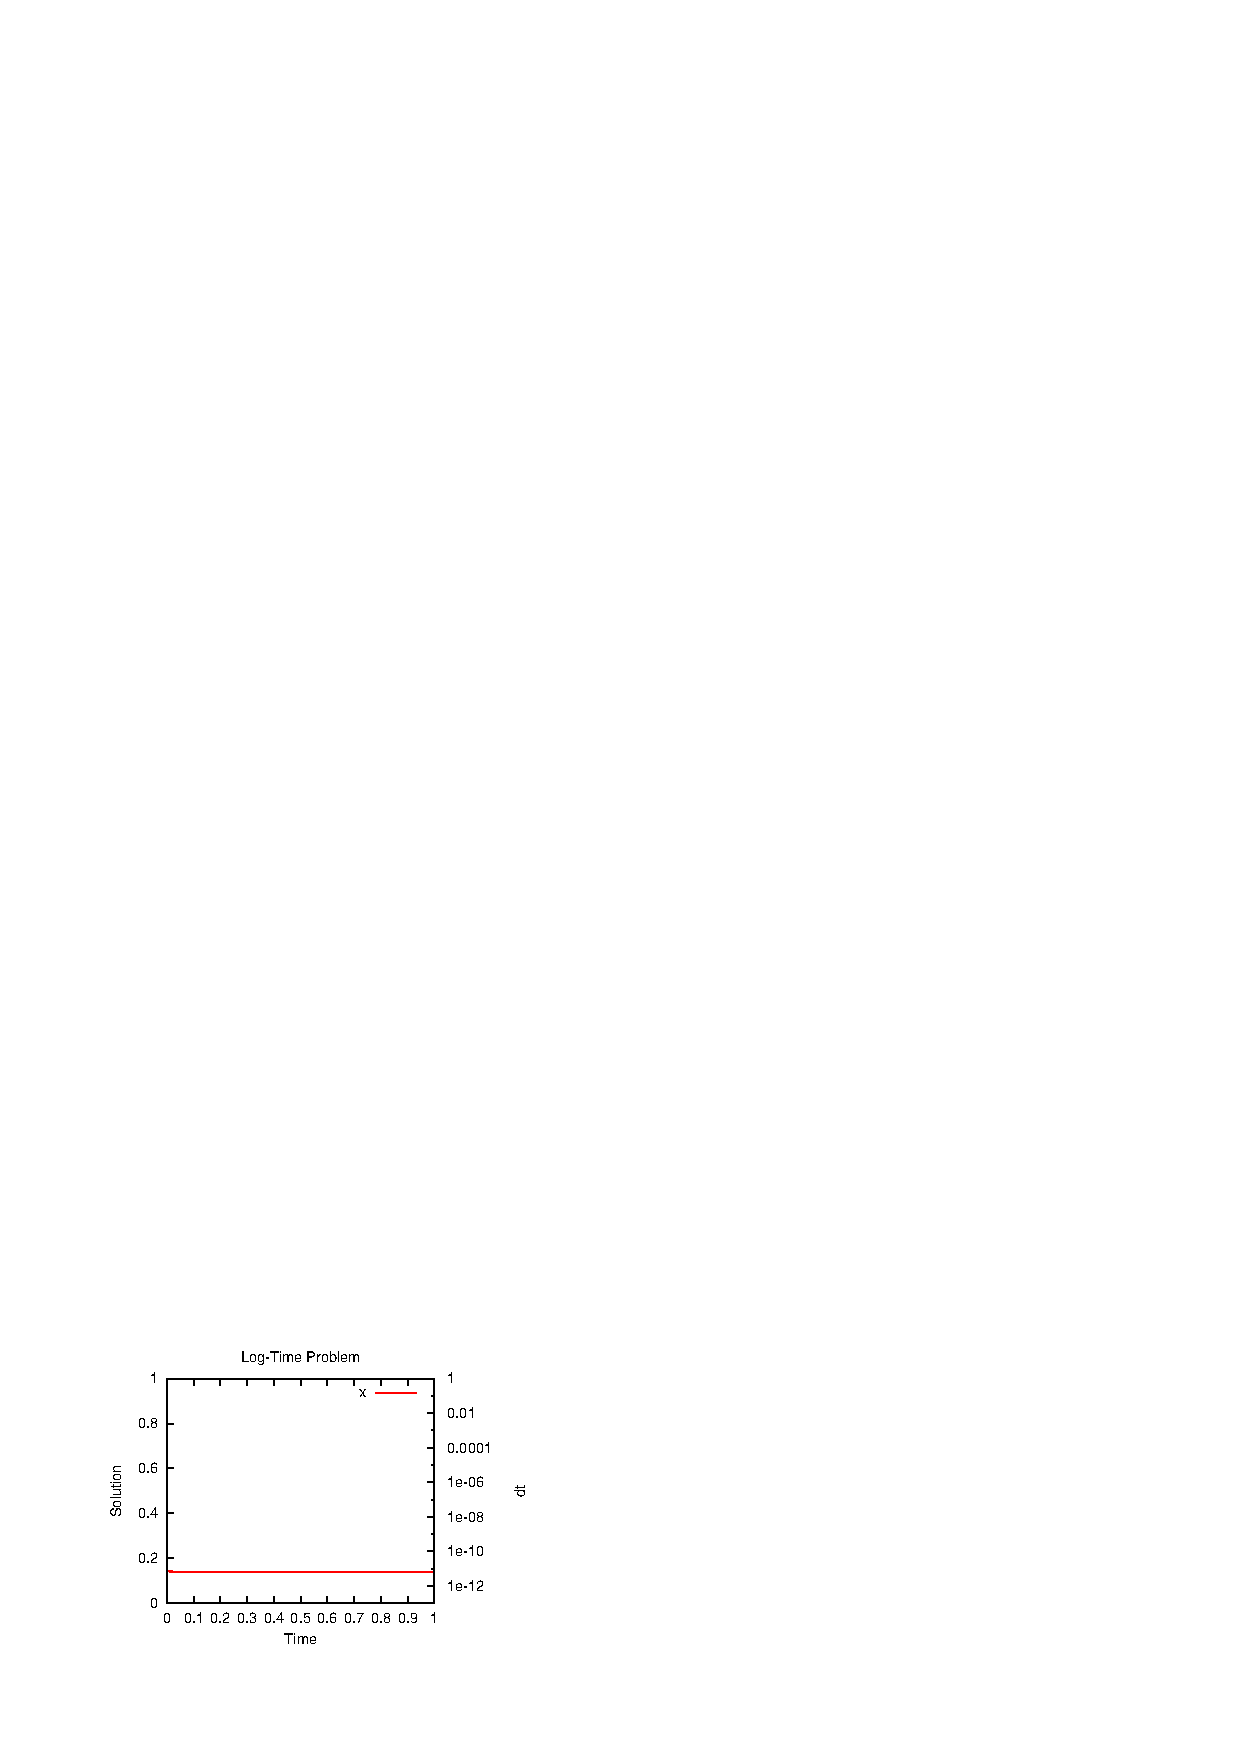
\includegraphics[width=2.75in]{figures/logtime-linear}\tabularnewline
\end{tabular}\caption{Exact solution to the Log-Time problem with a) logarithmic x-axis
and b) linear x-axis.\label{rythmos:fig:LogTime-exact}}
\end{figure}
From Fig.~\ref{rythmos:fig:LogTime-exact}, one can see the challenge
to capture the strong transient for $10^{-10}\leq t<10^{-8}$ requiring
step sizes at least as small as $\Delta t=10^{-11}$, and then transition
to larger and larger time steps as $t\rightarrow1$ to reduce the
overall computational costs.

The ODE for this problem is
\[
x(t)=\frac{a\left(bt^{4}+ct^{9/2}\right)}{\left(b+\sqrt{t}\right)\left(d+t^{4}\right)}
\]
where $a=1.4$, $b=0.0001$, $c=0.1$, $d=10^{-36}$, and the initial
condition is $x(0)=0.$ The center of the rapid increase is approximately
$d^{1/4}$, the product $ac$ sets the steady state value, and the
center of the decay is approximately $b^{2}$. The time derivative
is given by
\[
\dot{x}=\frac{at^{3}\left(8b^{2}d+b\sqrt{t}\left((9c+7)d+(c-1)t^{4}\right)+8cdt\right)}{2\left(b+\sqrt{t}\right)^{2}\left(d+t^{4}\right)^{2}}.
\]

